\section{Effective Strain Calibration}

For strain coefficient calibration we assume idealized basins with  different materials including a rock half space, dense sediment and loose sediment inside the basin. We only allow the materials inside the basin to behave nonlinear or equivalent linear.  In the first attempt we assume that only shear strains are dominant and effective. Therefore, we use the following equation.

 \begin{equation}
 \gamma_{max} = G(A \gamma_{xy}^{2} + B\gamma_{xz}^{2} + C\gamma_{yz}^{2} )^H
 \end{equation}


 We use a point source model with seismic moment corresponding to $Mw=4.5$. Fig.~\ref{fig:study_region} show the basin, epicenter, and stations location. 

\begin{figure}[H]
    \centering
    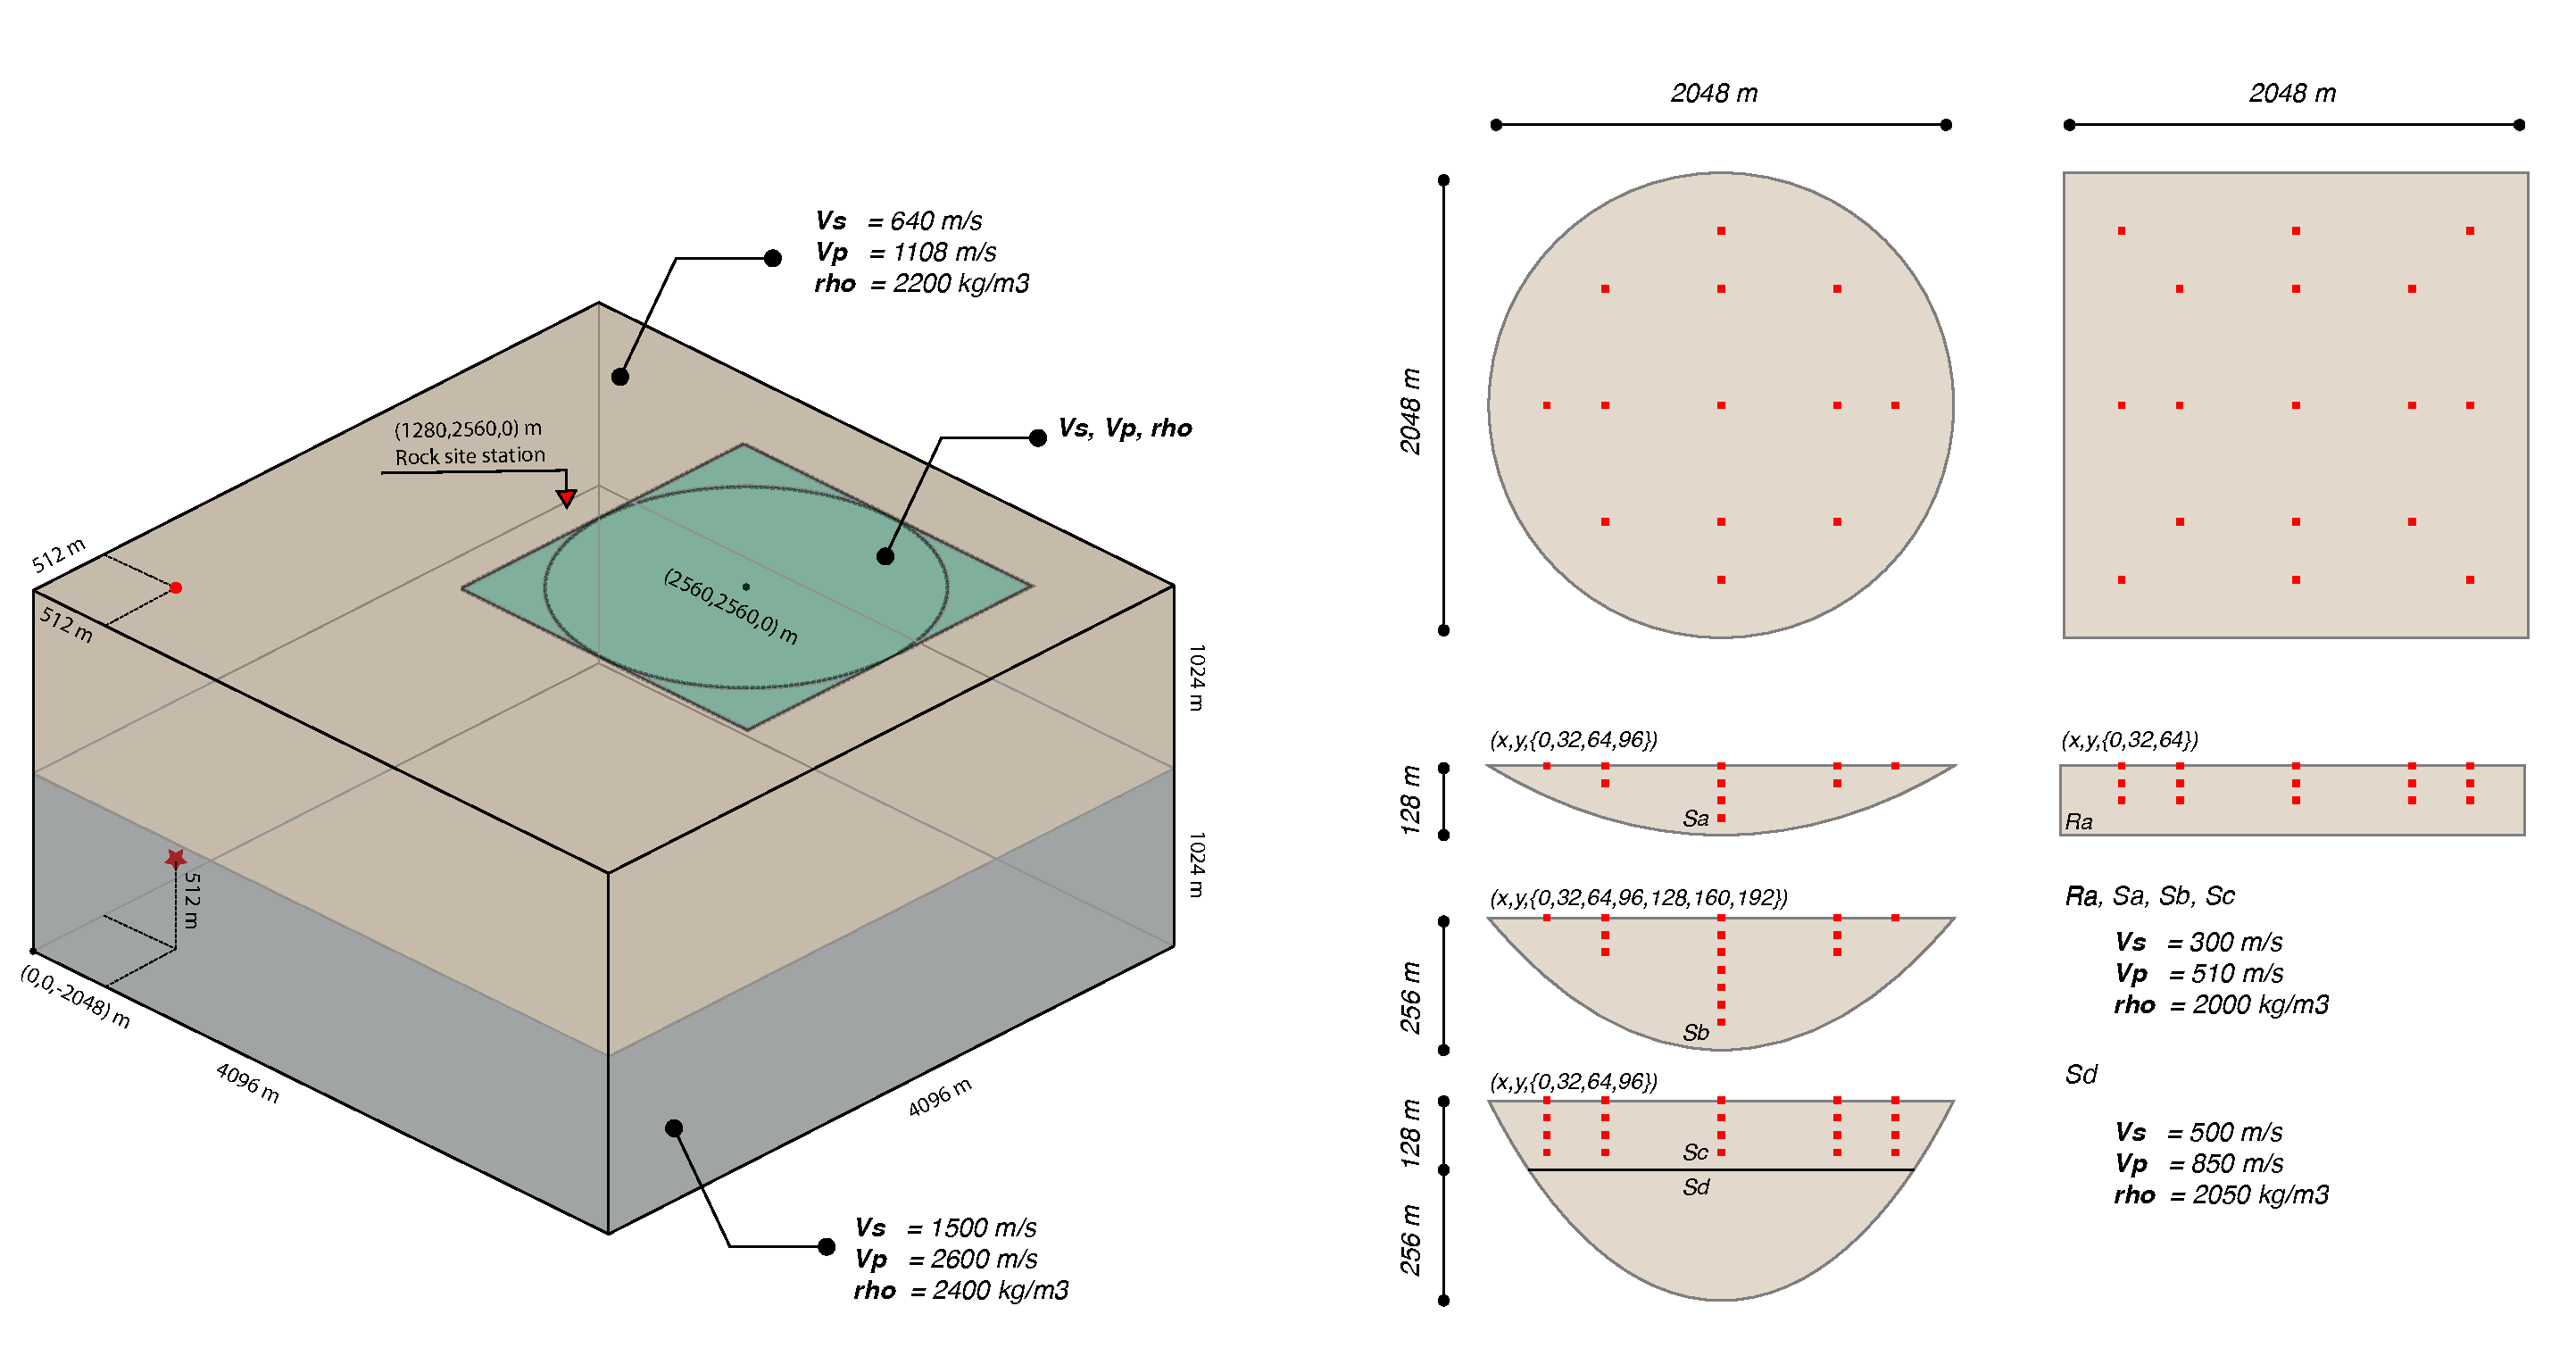
\includegraphics[width=\textwidth]{figures/pdf/study_region.pdf}
    \caption{Idealized basins for effective strain calibration}
    \label{fig:study_region}
\end{figure}


\subsection{Nonlinear Simulation}

Equivalent linear method is an approach to approximate the fully nonlinear method. The damping and shear modulus reduction curve with respect to strain are two extra inputs for adding to linear simulation to conduct equivalent linear method. In this study, in order to make sure that the calibration of the effective strain level based on comparing the results with fully nonlinear simulation. The fully nonlinear simulation, which is used in this study, is based on vonMises model with Modified Frederich-Armstrong formulation. We extract the shear modulus reduction and damping curve for the model and use it as an input values in the equivalent linear model. 

\subsubsection{von Mises Modified Frederich-Armstrong formulation}

For nonlinear constitutive model we use Modified Frederich-Armstrong formulation. No elastic region is considered, thus Gamma=0. The modification generates closed hysteric loops.

\subsubsection{Shear Modulus degradation and Damping}

We numerically extracted shear modulus degradation and damping curves from von Mises Modified Frederich-Armstrong formulation for the following soil materials:

\begin{itemize}
\item Elastic limit (k) = 0
\item Undrained strength (Su) = 70 $KN$
\item Material parameter to adjust (psi) = 100
\item S-wave velocity (Vs) = 300 $m/s$
\item Poisson's ration ($\mu$)=0.3
\item Density ($\rho$) = 2000 $kg/m^3$
\end{itemize}

Fig.~\ref{fig:GD_18_points_FAM_su70kn_psi100_vs300} shows the shear modulus degradation and damping curve. 

 \begin{figure}[H]
    \centering
    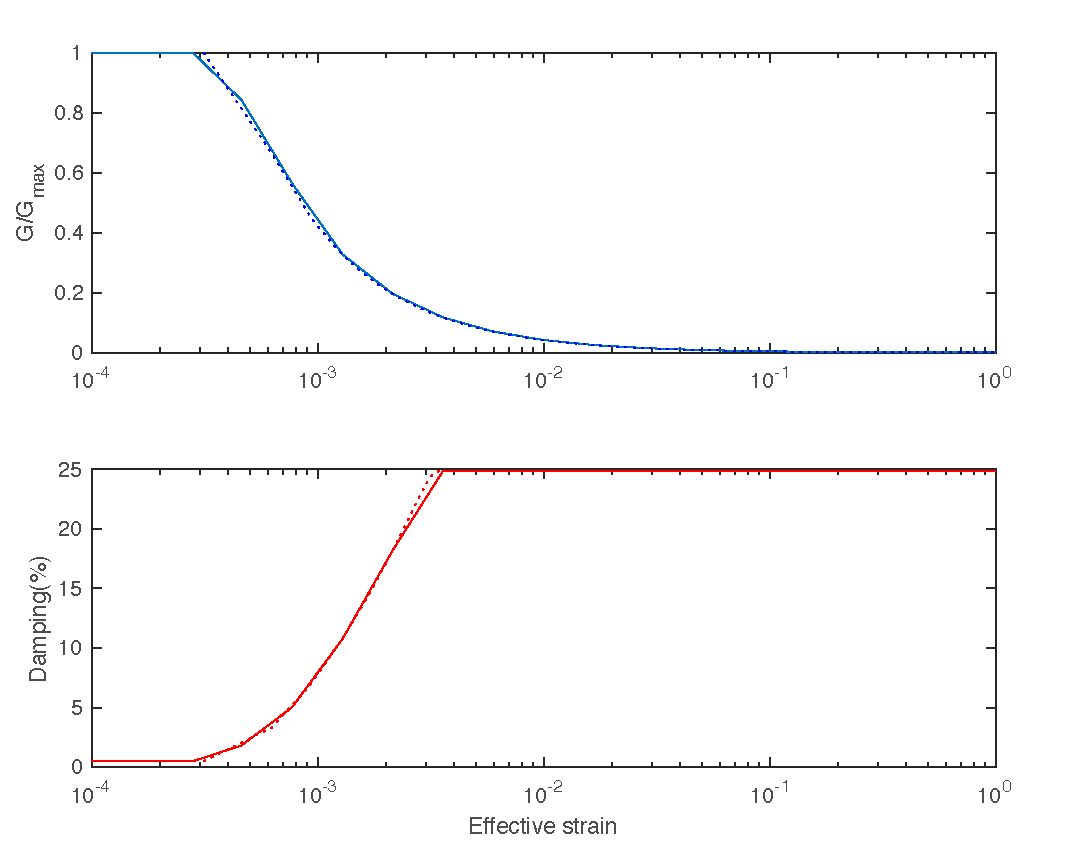
\includegraphics[width=300px]{figures/pdf/GD_18_points_FAM_su70kn_psi100_vs300.pdf}
    \caption{Variation of shear modulus and damping for the study soil material with based on effective strain level. Dashed-line is the original value based on 4000 numerical values. The solid line represents the interpolated values for 18 points.}
    \label{fig:GD_18_points_FAM_su70kn_psi100_vs300}
\end{figure}

%% source model

\subsection{Source Model}

In this study, in order to calibrate the nonlinear simulation and equivalent simulation we used a point source. In order to reduce the effect of permanent displacement at the final results we defined the source slip function as a combination of Ricker pulses. Fig.~\ref{fig:slip_function} represent the source slip function. 

 \begin{figure}
    \centering
    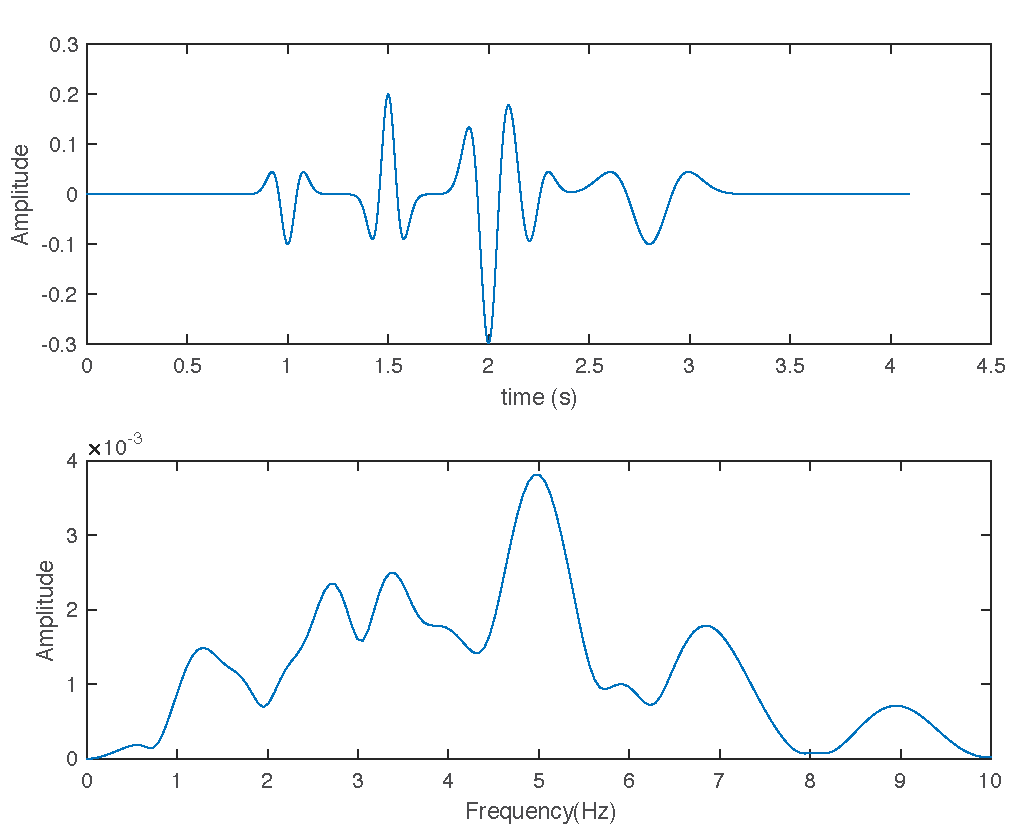
\includegraphics[width=300px]{figures/pdf/slip_function.pdf}
    \caption{Point source slip function}
    \label{fig:slip_function}
\end{figure}








%% parameters calibration

\subsection{Parameters Calibration}

In order to calibrate the effective strain parameters (A,B,C,G, and H) we compare the results of simulation with nonlinear soil effect and equivalent linear soil effect with different parameters for four different configuration of basins and two different point sources. Fig.~\ref{fig:comparison_linear_nonlinear} represents and example of comparison between nonlinear and linear simulation for a station at the surface and the middle of basin. 

 \begin{figure}[H]
    \centering
    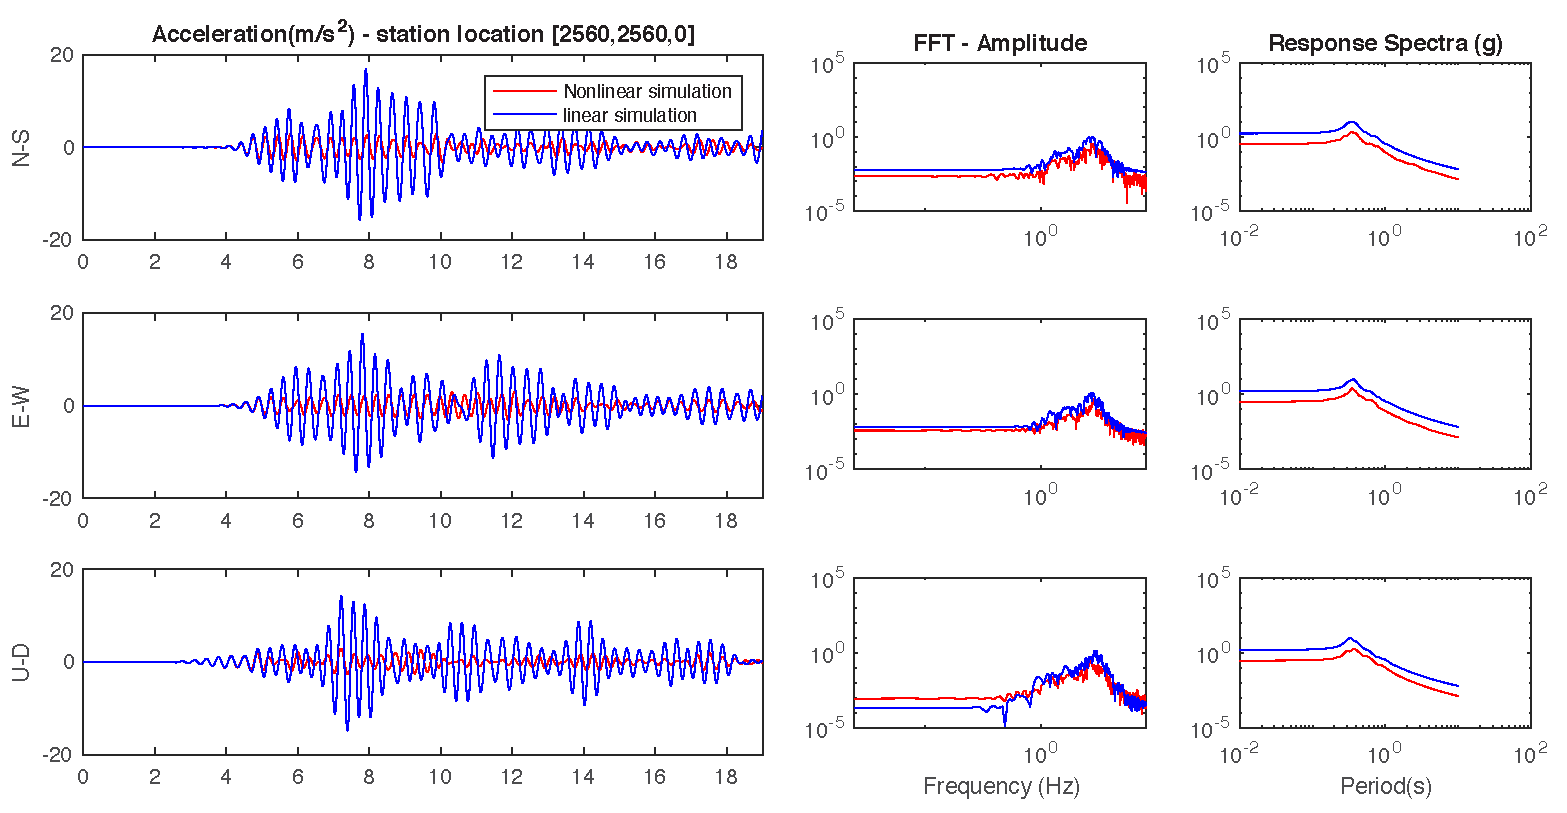
\includegraphics[width=\textwidth]{figures/pdf/comparison_linear_nonlinear.pdf}
    \caption{Comparison between nonlinear and linear simulation for station at the surface in the middle of the basin for spherical basin 3 and point source 2.}
    \label{fig:comparison_linear_nonlinear}
\end{figure}

Fig.~\ref{fig:stress_strain_b3_p2_st2560_2560_96} represents the stress-strain relationship for different components of the a station in the middle of the basin at the depth of 96 m. 

 \begin{figure}[H]
    \centering
    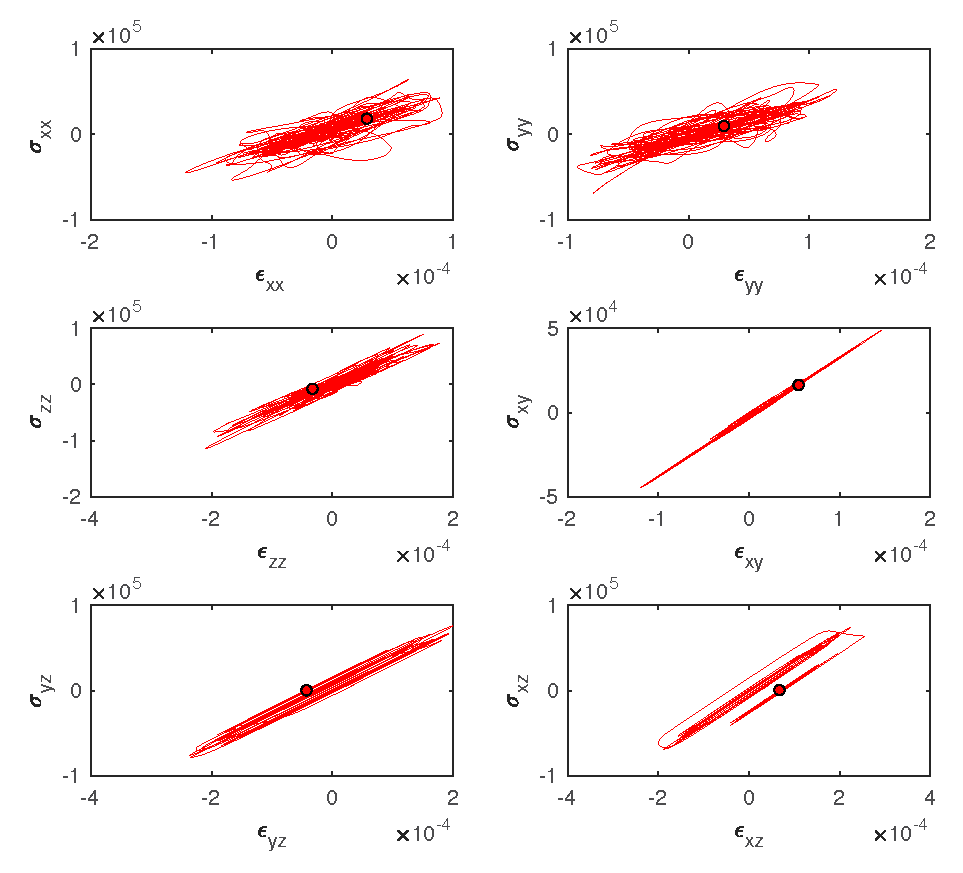
\includegraphics[width=\textwidth]{figures/pdf/stress_strain_b3_p2_st2560_2560_96.pdf}
    \caption{Stress-strain relationship for station at the depth of 96 m in the middle of the basin for spherical basin 3 and point source 2.}
    \label{fig:stress_strain_b3_p2_st2560_2560_96}
\end{figure}


Fig.~\ref{fig:iteration_test_value_convergence} represents the convergence in time and frequency and response spectra for different iteration of equivalent linear simulation.  

 \begin{figure}[H]
    \centering
    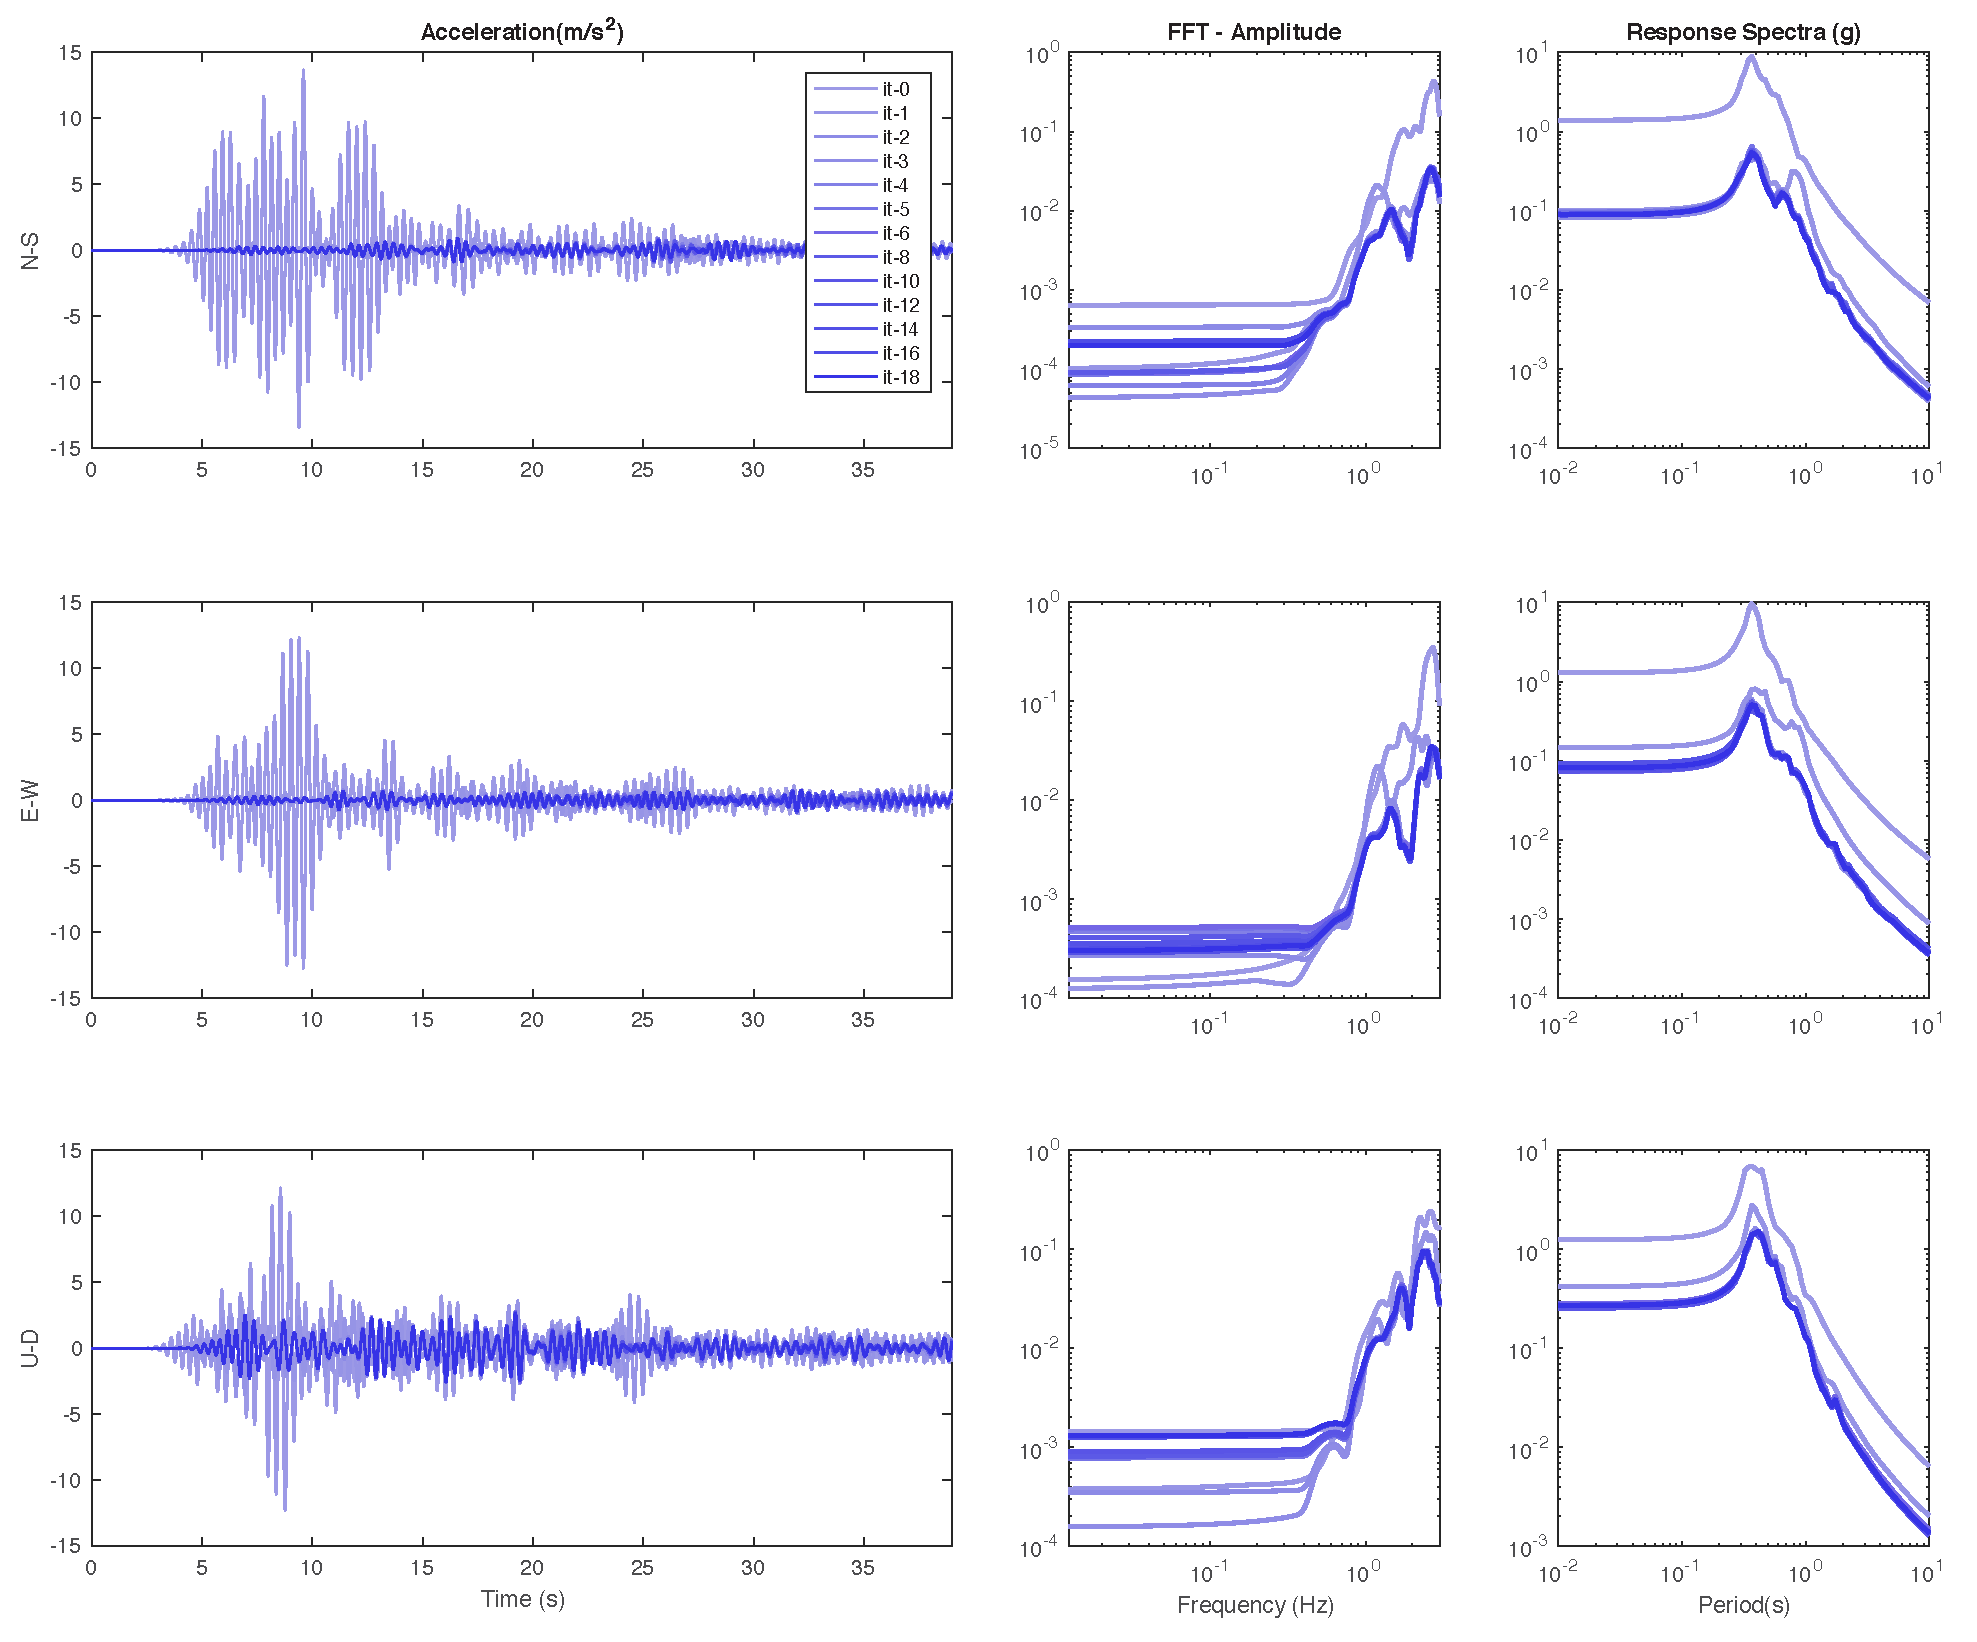
\includegraphics[width=\textwidth]{figures/pdf/iteration_test_value_convergence.pdf}
    \caption{Stress-strain relationship for station at the depth of 96 m in the middle of the basin for spherical basin 3 and point source 2.}
    \label{fig:iteration_test_value_convergence}
\end{figure}

Obviously with modifying effective strain parameters, the results change. Among different parameters, some of them give perfect match with nonlinear, and some other gives different results. For example Fig.~\ref{fig:match_spherical_basin_3_point_source_2_HC_eqlinear_c13_2560_3072_96} shows an acceptable match for the horizontal components whereas equivalent linear method gives higher values for vertical component. The shift in arrival time in equivalent linear method is expectable. Equivalent linear method starts with reduced shear modulus shear wave velocity, which cause delay in wave propagation. 

 \begin{figure}[H]
    \centering
    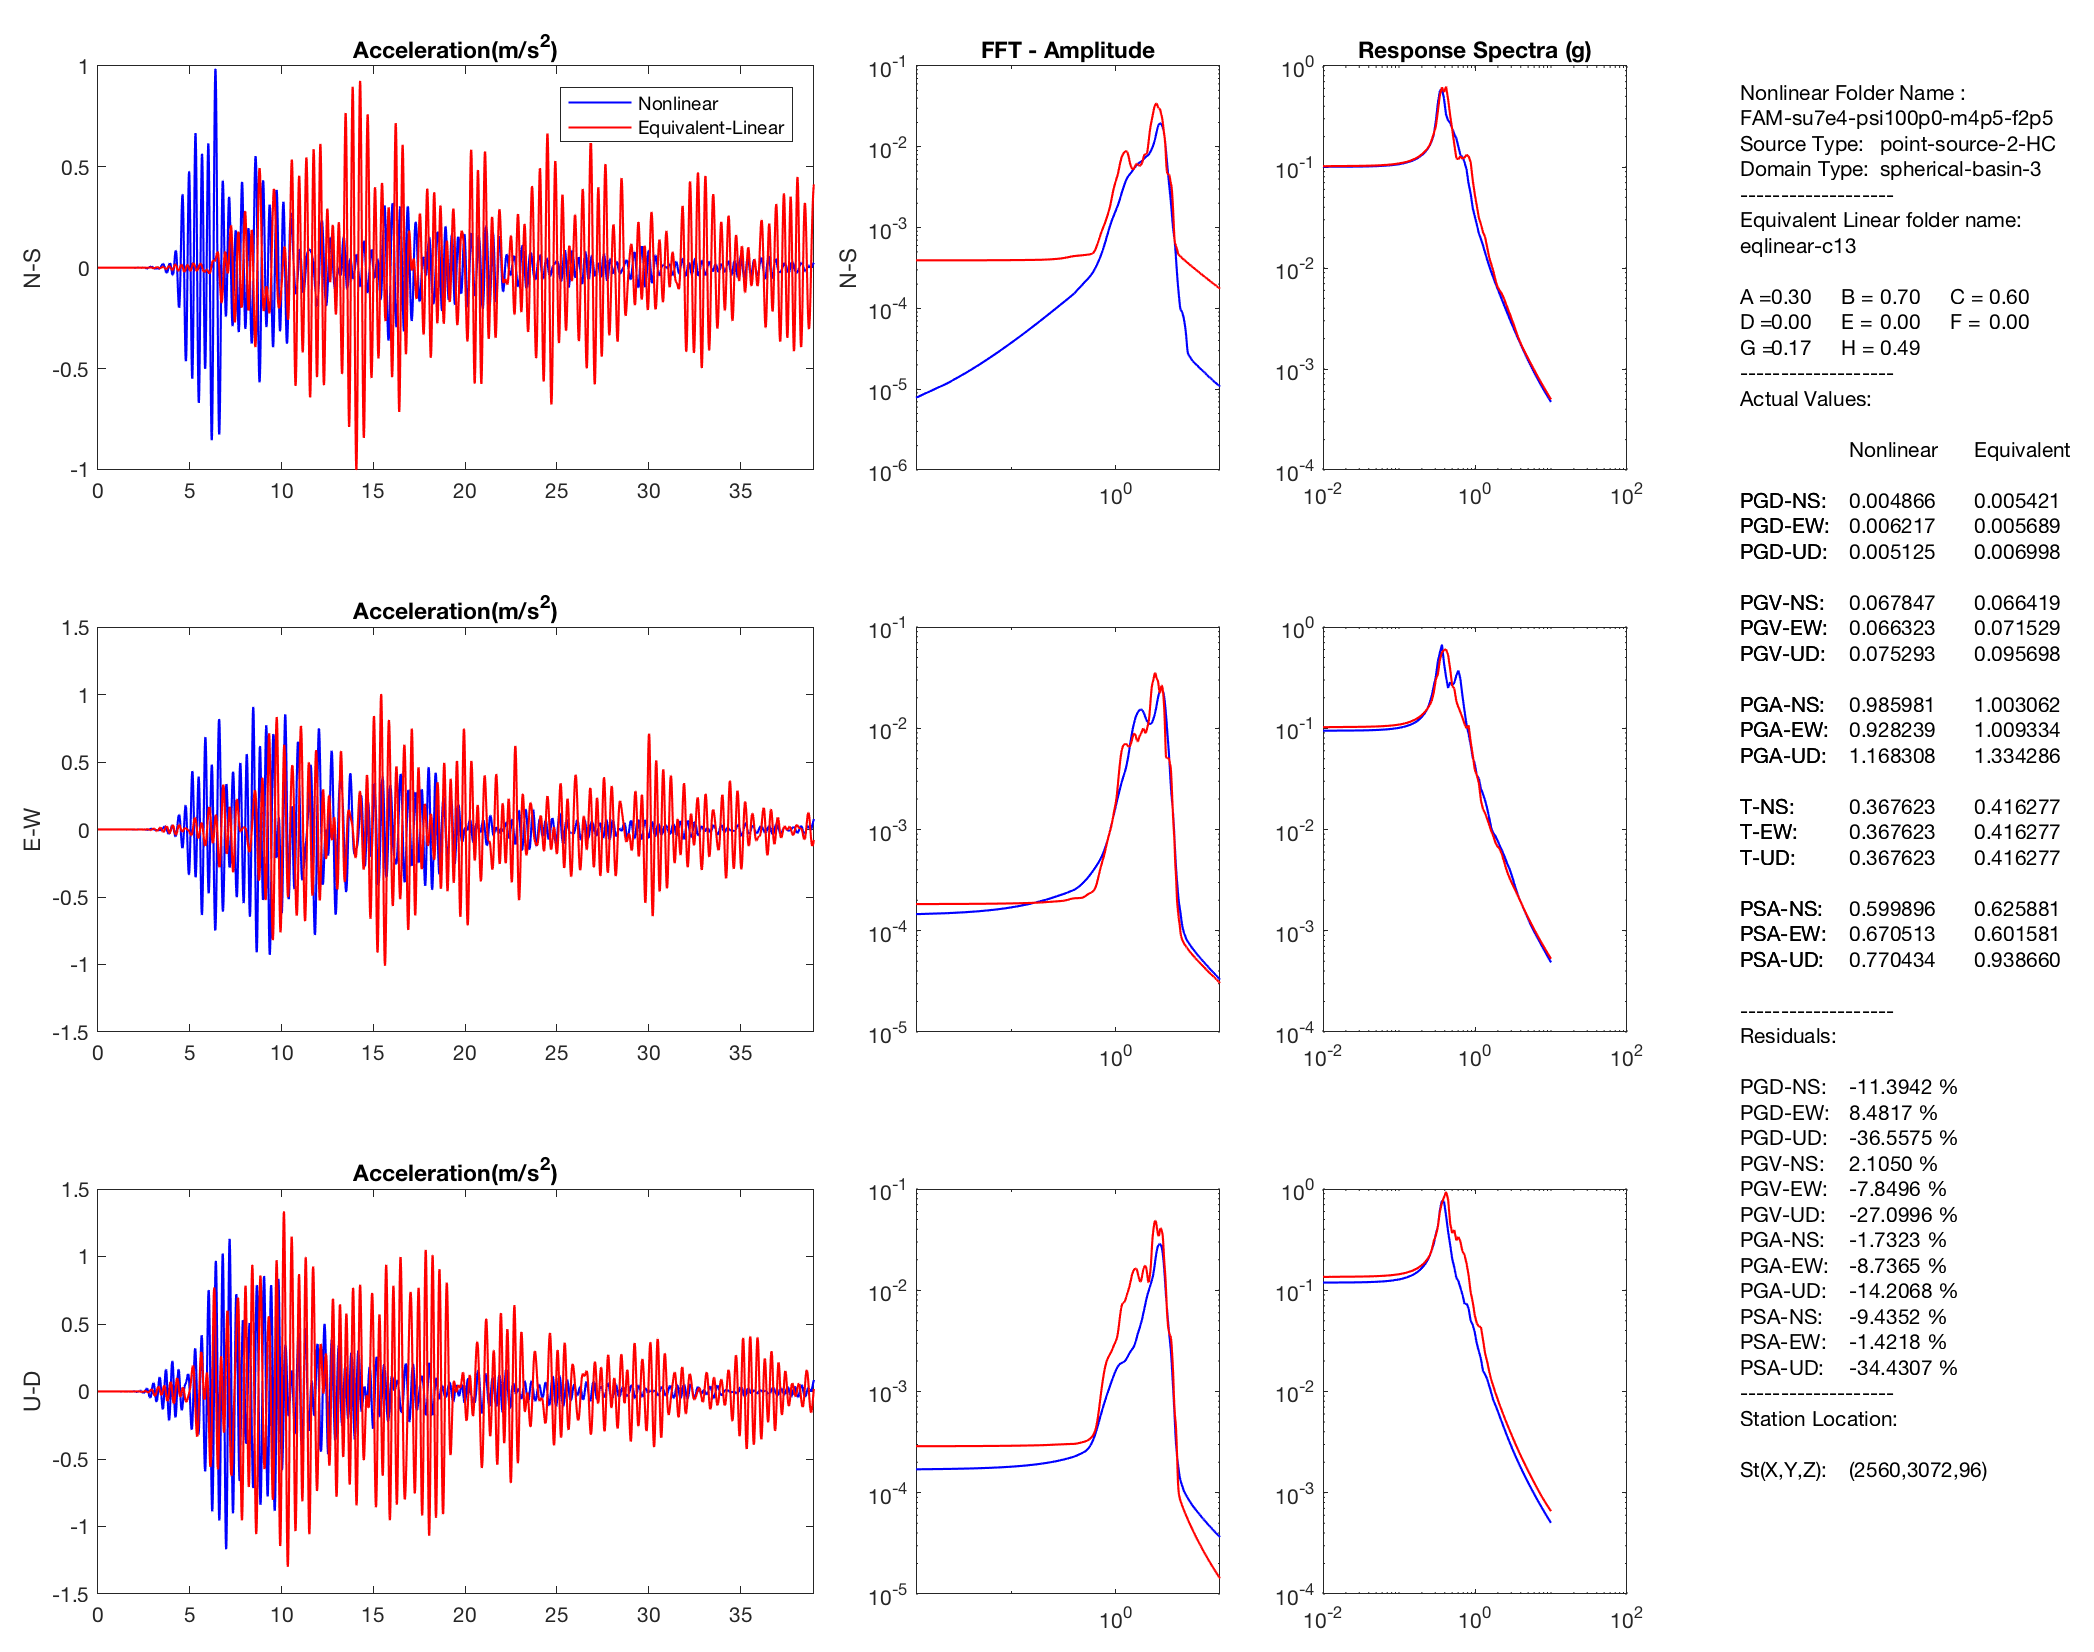
\includegraphics[width=\textwidth]{figures/pdf/match_spherical_basin_3_point_source_2_HC_eqlinear_c13_2560_3072_96.pdf}
    \caption{An example of comparison between equivalent linear and nonlinear simulation.}
    \label{fig:match_spherical_basin_3_point_source_2_HC_eqlinear_c13_2560_3072_96}
\end{figure}

 Fig.~\ref{fig:element_stress_strain} shows an stress tensors for a schematic element. 

 \begin{figure}[H]
    \centering
    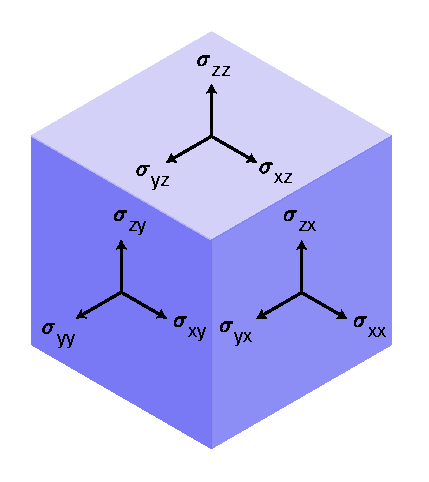
\includegraphics[width=100 px]{figures/pdf/element_stress_strain.pdf}
    \caption{A schematic view of element and its stress tensors. x,y, and z are corresponding to 1,2, and 3.}
    \label{fig:element_stress_strain}
\end{figure}


After conducting simulation for different parameters we take a look at data from different perspective. For us it is important to understand that what kind of effects we can expect from variation of different parameters. Fig.~\ref{fig:A_var_BC_1_H0p5_G0p25},~\ref{fig:B_var_AC1_H0p5_G0p25},~\ref{fig:C_var_AB1_H0p5_G0p25},~\ref{fig:G_var_ABC1_H0p6},~\ref{fig:H_var_ABC1_G0p25}, represent the variation of residuals with variation of A, B, C, G, and H, where other parameters are kept constant. 

 \begin{figure}[H]
    \centering
    \includegraphics[width=\textwidth]{figures/pdf/A_var_BC_1_H0p5_G0p25.pdf}
    \caption{Variation of residuals for different A values. Other parameters kept constant.}
    \label{fig:A_var_BC_1_H0p5_G0p25}
\end{figure}

 \begin{figure}[H]
    \centering
    \includegraphics[width=\textwidth]{figures/pdf/B_var_AC1_H0p5_G0p25.pdf}
    \caption{Variation of residuals for different B values. Other parameters kept constant.}
    \label{fig:B_var_AC1_H0p5_G0p25}
\end{figure}

 \begin{figure}[H]
    \centering
    \includegraphics[width=\textwidth]{figures/pdf/C_var_AB1_H0p5_G0p25.pdf}
    \caption{Variation of residuals for different C values. Other parameters kept constant.}
    \label{fig:C_var_AB1_H0p5_G0p25}
\end{figure}

 \begin{figure}[H]
    \centering
    \includegraphics[width=\textwidth]{figures/pdf/G_var_ABC1_H0p6.pdf}
    \caption{Variation of residuals for different G values. Other parameters kept constant.}
    \label{fig:G_var_ABC1_H0p6}
\end{figure}

 \begin{figure}[H]
    \centering
    \includegraphics[width=\textwidth]{figures/pdf/H_var_ABC1_G0p25.pdf}
    \caption{Variation of residuals for different H values. Other parameters kept constant.}
    \label{fig:H_var_ABC1_G0p25}
\end{figure}

G and H has an overall effect. It is obvious that lower G value and higher H value will decrease the effective strain and reduce the nonlinearity effects. From figures it is obvious that results are different for different depth. However, we cannot observe depth dependent pattern. They are different for different depth because of different strain level that they experience during loading. The reason is the jumps between different depth which are not following decreasing or increasing in depth trend. For example in Fig.~\ref{fig:C_var_AB1_H0p5_G0p25} for NS component depth of 0 and 96 have positive residuals, however, depth of 32 and 64 have negative residuals. It shows at surface and close to the boundary of basin-bedrock higher strain level put more nonlinearly on elements and they result in small amplitudes than nonlinear simulation and therefore, they have positive residuals. So what we are dealing here is pure strain level at each element.  Also, according to these figures we can say that variation of A, B, and C, at this level, do not have significant effects on the results.  Obviously G and H can have similar effect and we can define a relationship between them to give us the least residuals. 

Fig.~\ref{fig:all_data_residulas_response} represents all data residuals (51900 data). It seems, in general, horizontal components are easy to fit than vertical components. The vertical component tends to have negative residuals which means the results are underdamped in equivalent linear method for UD component. 

 \begin{figure}[H]
    \centering
    \includegraphics[width=\textwidth]{figures/pdf/all_data_residulas_response.pdf}
    \caption{Residuals of response spectra for different components. All test data are involved (51900).}
    \label{fig:all_data_residulas_response}
\end{figure}

We narrow our look and analyze data in $-0.1 to 0.1$ residuals, which represents the 10\% (actual value 0.0953) difference than nonlinear simulation. 158 data points are in this range. Among them 20, 124, 11, and 3 are at depth of 0, 32, 64, and 96. Data include all source types and basin configuration.  It seems variation of G and H is the most important values to consider. Fig.~\ref{fig:variation_G_H} shows the variation of G and H for those stations that have less than 0.1 residuals for response spectra in all components. 

 \begin{figure}[H]
    \centering
    \includegraphics[width=\textwidth]{figures/pdf/variation_G_H.pdf}
    \caption{Variation of G and H and 3rd degree polynomials as fitting functions. positive is the sign of residual.}
    \label{fig:variation_G_H}
\end{figure}

As we discussed earlier, we defined a polynomial to generate a regression line between G and H. G and H has similar effect on effective strain and we expect to see the same effective strain for any related G and H. In order to understand if the results are fairly stable with different G and H values, we use the current G and H relationship and generate H based on different values of G for 10000 random strain level. We expect to see similar mean and standard deviation for any G value, given the fact that we generate the H value based on each G values. Fig.\ref{fig:Gh_sensitivity_plot} represent the results. 

 \begin{figure}[H]
    \centering
    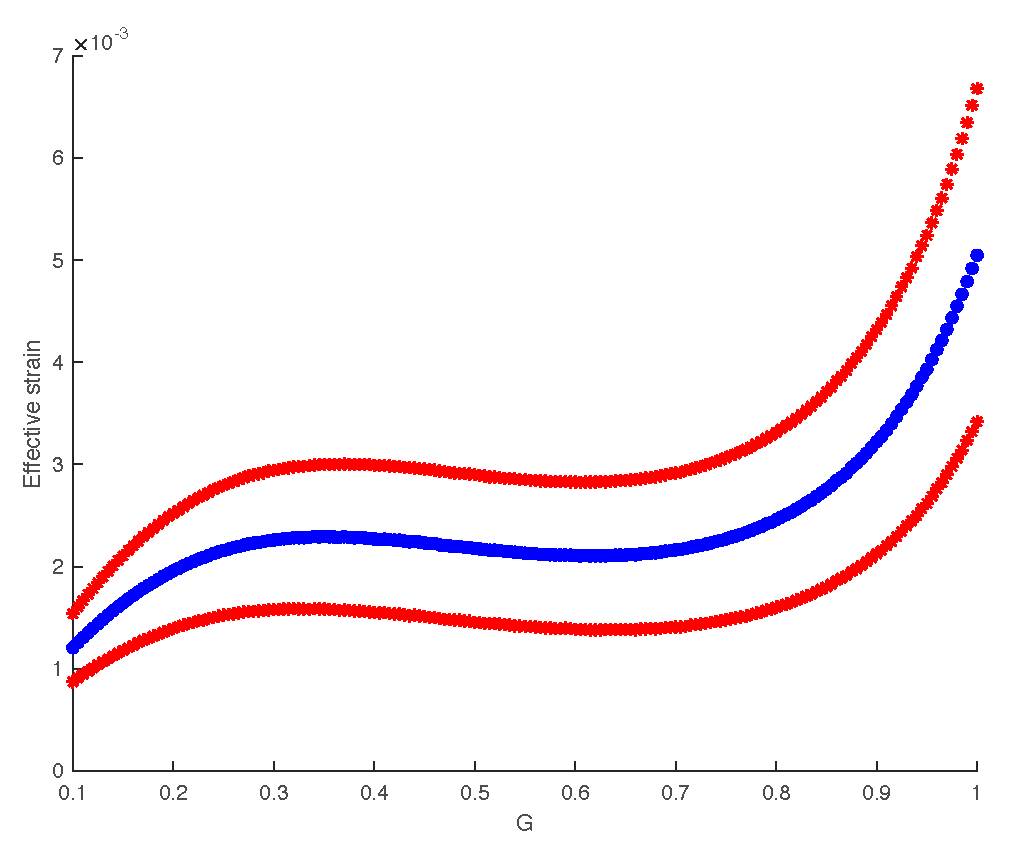
\includegraphics[width=300 px]{figures/pdf/Gh_sensitivity_plot.pdf}
    \caption{Variation of G and effective strain. Blue dots are mean and red dots are one standard deviation for 10000 different combination of strains. The results suggest that G should be kept between 0.25 and 0.75 in order to get stable effective strain.}
    \label{fig:Gh_sensitivity_plot}
\end{figure}

According to the figure, for G less than 0.25 in general we get smaller effective strain and for G higher than 0.75 we get bigger effective strain. It remains fairly stable between 0.25 and 0.75.  We test three G (0.3,0.5,0.7) and their corresponding H values. We expect the results be the same, however they are slightly different. One obvious reason for this can be not accurate regression line. Figure~\ref{fig:Gh_sensitivity_plot} shows a comparison for a station at the surface. We also conclude the stable domain for G based on 10000 random combination. In result, we can accept small differences. 

 \begin{figure}[H]
    \centering
    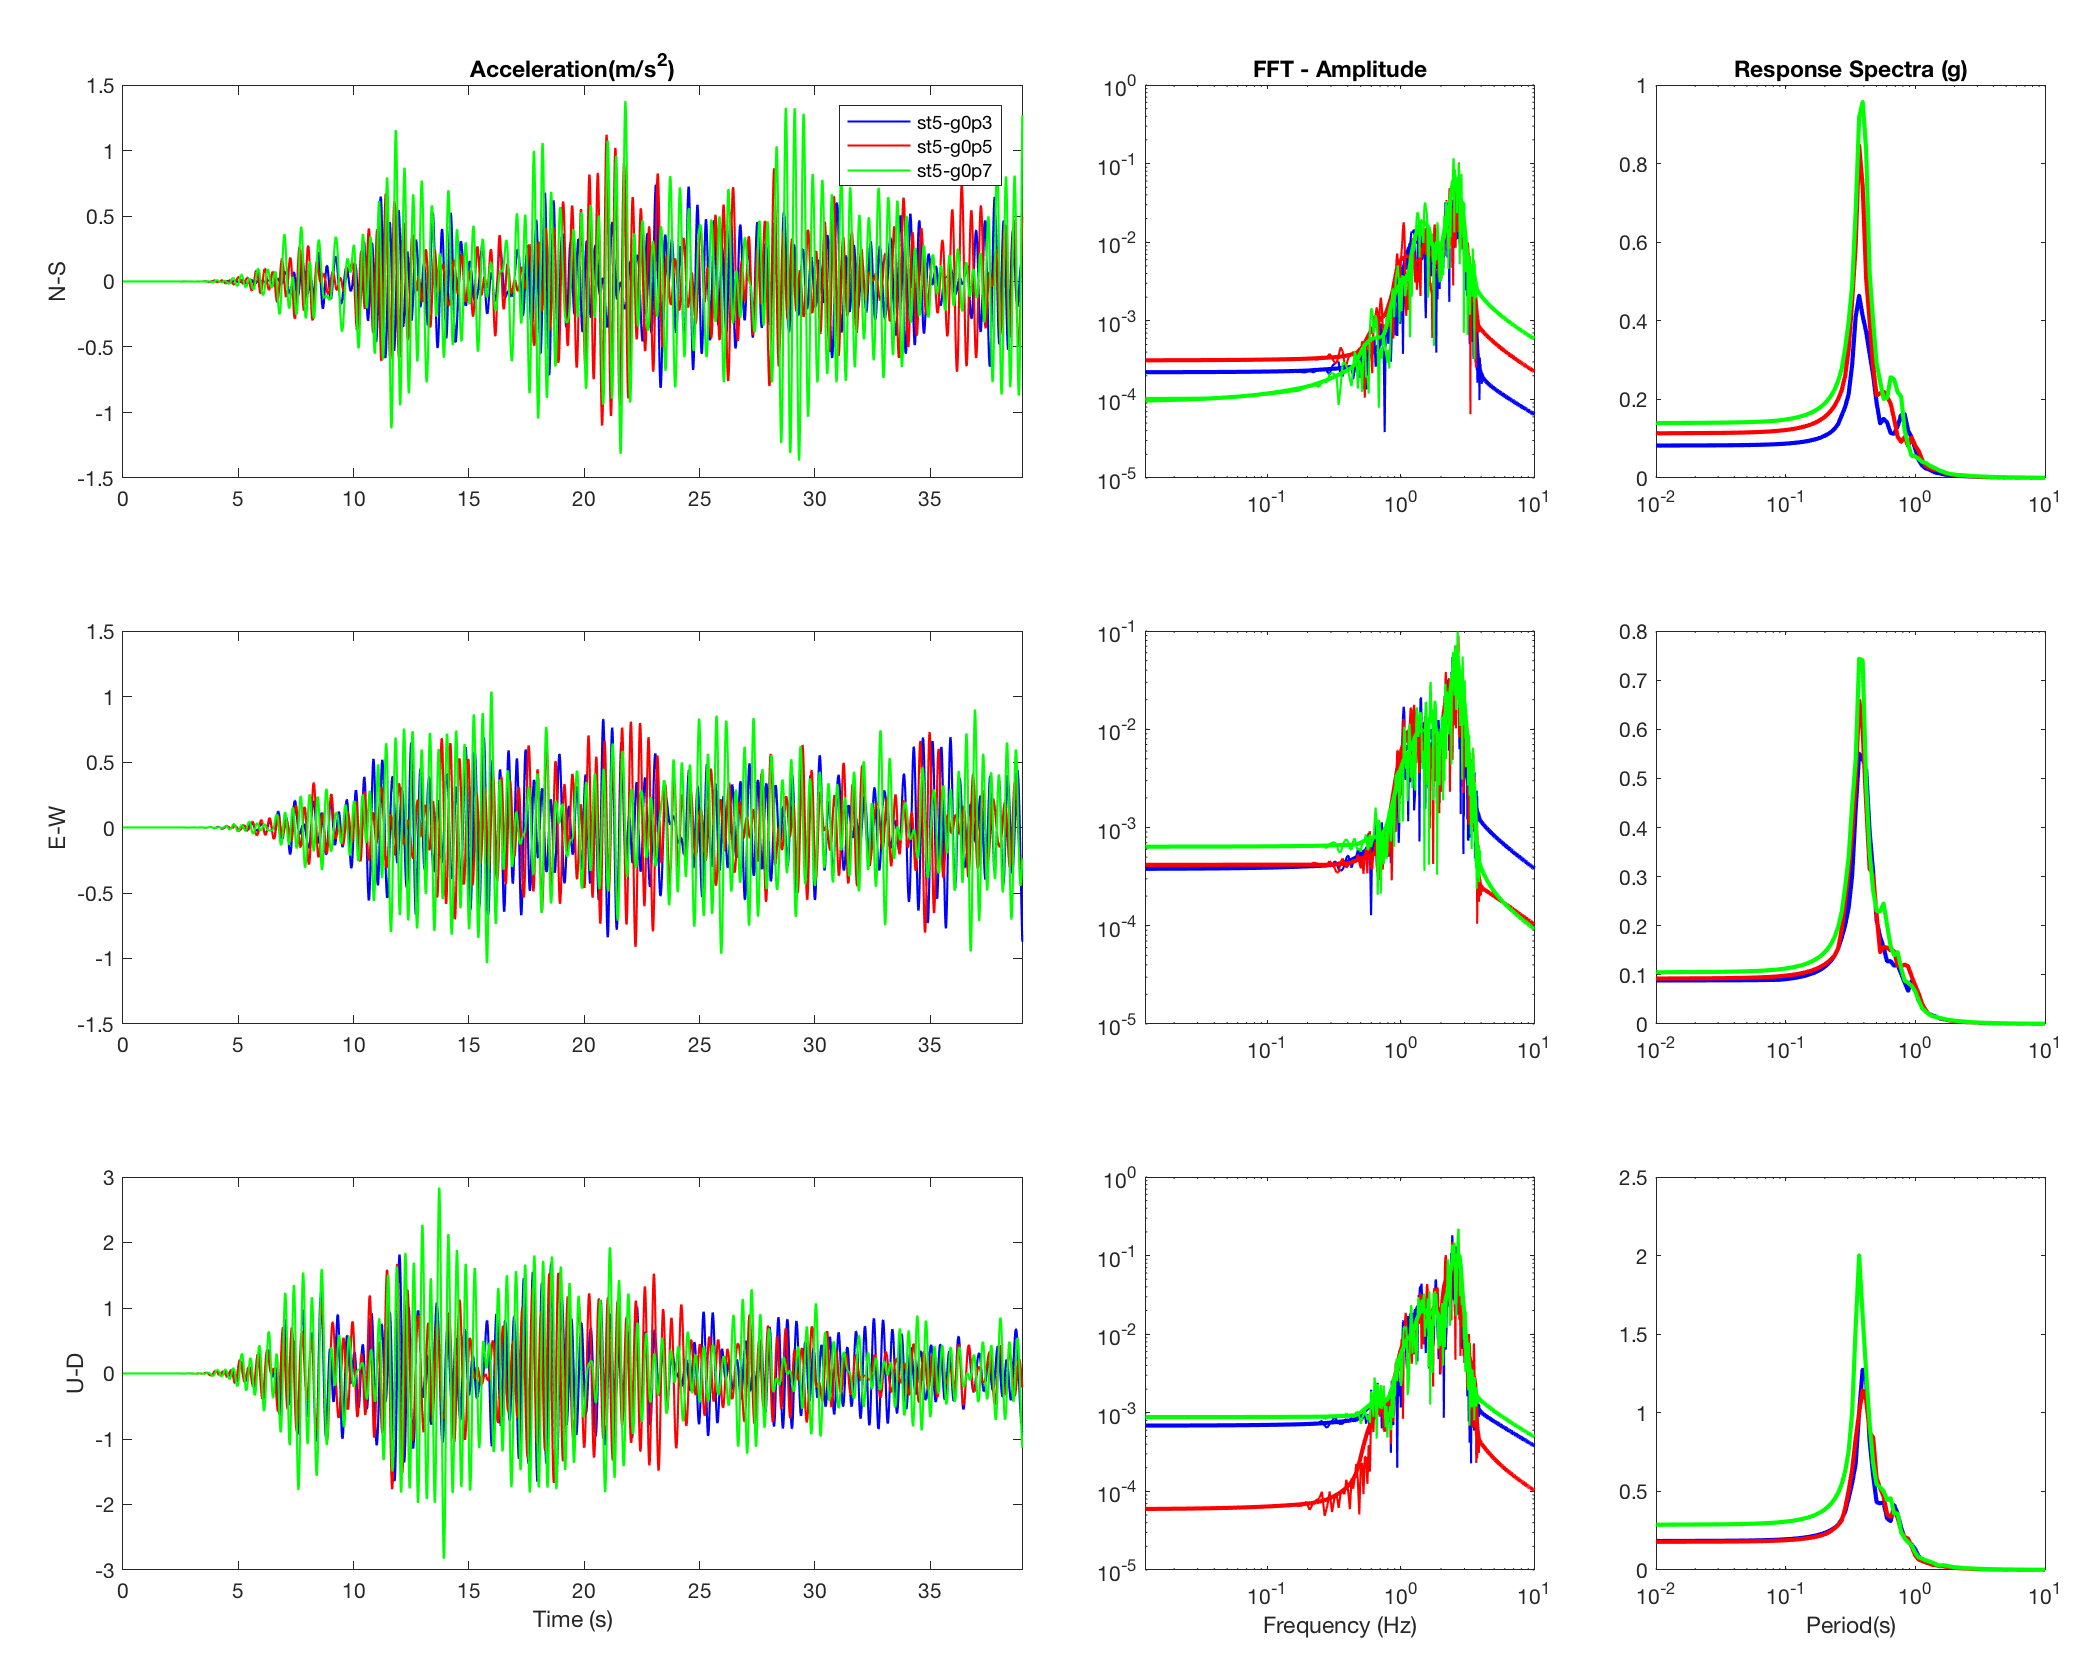
\includegraphics[width=300 px]{figures/pdf/GH_var_test_station_surface_middle_basin.pdf}
    \caption{Comparison of results for a station at the surface with different G value. H value computed according to the Fig.~\ref{fig:variation_G_H} regression line. According to Fig. \ref{fig:Gh_sensitivity_plot} all three parameters are supposed to give fairly close effective strains. }
    \label{fig:GH_var_test_station_surface_middle_basin}
\end{figure}


















